\documentclass[twoside]{article}
\setlength{\oddsidemargin}{0.25 in}
\setlength{\evensidemargin}{-0.25 in}
\setlength{\topmargin}{-0.6 in}
\setlength{\textwidth}{6.5 in}
\setlength{\textheight}{8.5 in}
\setlength{\headsep}{0.75 in}
\setlength{\parindent}{0 in}
\setlength{\parskip}{0.1 in}
\newcommand{\eqdef}{:\mathrel{\mathop=}}
\newcommand{\norm}[1]{\left\lVert #1 \right\rVert}

%
% ADD PACKAGES here:
%

\usepackage{amsmath,amsfonts,graphicx}

%
% The following commands set up the lecnum (lecture number)
% counter and make various numbering schemes work relative
% to the lecture number.
%
\newcounter{lecnum}
\renewcommand{\thepage}{\thelecnum-\arabic{page}}
\renewcommand{\thesection}{\thelecnum.\arabic{section}}
\renewcommand{\theequation}{\thelecnum.\arabic{equation}}
\renewcommand{\thefigure}{\thelecnum.\arabic{figure}}
\renewcommand{\thetable}{\thelecnum.\arabic{table}}

%
% The following macro is used to generate the header.
%
\newcommand{\lecture}[4]{
   \pagestyle{myheadings}
   \thispagestyle{plain}
   \newpage
   \setcounter{lecnum}{#1}
   \setcounter{page}{1}
   \noindent
   \begin{center}
   \framebox{
      \vbox{\vspace{2mm}
    \hbox to 6.28in { {\bf Advanced Machine Learning
	\hfill Fall 2020} }
       \vspace{4mm}
       \hbox to 6.28in { {\Large \hfill Lecture #1: #2  \hfill} }
       \vspace{2mm}
       \hbox to 6.28in { {\it  #3 \hfill  #4} }
      \vspace{2mm}}
   }
   \end{center}
   \markboth{Lecture #1: #2}{Lecture #1: #2}

   {\bf Note}: {\it LaTeX template courtesy of UC Berkeley EECS dept.}

   {\bf Disclaimer}: {\it These notes are adapted from ETH's Advanced Machine Learning Course, Cornell's CS4780 Course, "The Element of Statistical Learning" and "Boosting: Foundations and Algorithms" books.}
   \vspace*{4mm}
}
%
% Convention for citations is authors' initials followed by the year.
% For example, to cite a paper by Leighton and Maggs you would type
% \cite{LM89}, and to cite a paper by Strassen you would type \cite{S69}.
% (To avoid bibliography problems, for now we redefine the \cite command.)
% Also commands that create a suitable format for the reference list.
\renewcommand{\cite}[1]{[#1]}
\def\beginrefs{\begin{list}%
        {[\arabic{equation}]}{\usecounter{equation}
         \setlength{\leftmargin}{2.0truecm}\setlength{\labelsep}{0.4truecm}%
         \setlength{\labelwidth}{1.6truecm}}}
\def\endrefs{\end{list}}
\def\bibentry#1{\item[\hbox{[#1]}]}

%Use this command for a figure; it puts a figure in wherever you want it.
%usage: \fig{NUMBER}{SPACE-IN-INCHES}{CAPTION}
\newcommand{\fig}[3]{
			\vspace{#2}
			\begin{center}
			Figure \thelecnum.#1:~#3
			\end{center}
	}
% Use these for theorems, lemmas, proofs, etc.
\newtheorem{theorem}{Theorem}[lecnum]
\newtheorem{lemma}[theorem]{Lemma}
\newtheorem{proposition}[theorem]{Proposition}
\newtheorem{claim}[theorem]{Claim}
\newtheorem{corollary}[theorem]{Corollary}
\newtheorem{definition}[theorem]{Definition}
\newenvironment{proof}{{\bf Proof:}}{\hfill\rule{2mm}{2mm}}

% **** IF YOU WANT TO DEFINE ADDITIONAL MACROS FOR YOURSELF, PUT THEM HERE:

\newcommand\E{\mathbb{E}}

\begin{document}
%FILL IN THE RIGHT INFO.
%\lecture{**LECTURE-NUMBER**}{**DATE**}{**LECTURER**}{**SCRIBE**}
\lecture{9}{Ensemble Methods}{}{}
%\footnotetext{These notes are partially based on those of Nigel Mansell.}

% **** YOUR NOTES GO HERE:

% Some general latex examples and examples making use of the
% macros follow.  
%**** IN GENERAL, BE BRIEF. LONG SCRIBE NOTES, NO MATTER HOW WELL WRITTEN,
%**** ARE NEVER READ BY ANYBODY.


\section{Bagging} % Don't be this informal in your notes!
Suppose we fit a model to our training data $\mathcal{Z} = \{(x_{1},y_{1}),(x_{2},y_{2}),... ,(x_{n},y_{n})\}$, obtaining the prediction $\hat{f}(x)$ at input x. Bootstrap aggregation or bagging averages this prediction over a collection of bootstrap samples, thereby reducing its variance.
For each bootstrap sample $\boldsymbol{\mathcal{Z}}^{*b}, \; b = 1, 2,... ,B$, we fit our model, giving
prediction $\hat{f}^{*b}(x)$. The bagging estimate is defined by:
\begin{equation*}
    \hat{f}_{bag}(x) = \dfrac{1}{B} \sum_{b=1}^{B}\hat{f}^{*b}(x)
\end{equation*}


Bagging can dramatically reduce the variance of unstable procedures like trees, leading to improved prediction. A simple argument shows why bagging helps under squared-error loss, in short because averaging reduces variance and leaves bias unchanged.

\begin{theorem}

Assume our training observations $(x_{i},y_{i}), i = 1,... ,N $ are independently drawn from a distribution $\mathcal{P}$, and consider the ideal aggregate estimator $f_{ag}(x) = \mathbb{E}_{\mathcal{P}}[\hat{f}^*(x)]
$. Here $x$ is fixed and the bootstrap dataset $\boldsymbol{\mathcal{Z}^*}$
consists of observations $x_{i}^*,y_{i}^*, \;  i = 1, 2,... ,N$
sampled from $\mathcal{P}$.  Then:

\begin{equation*}
    \mathbb{E}_{\mathcal{P}}[Y - \hat{f}^*(x)]^2 = \mathbb{E}_{\mathcal{P}}[Y - \hat{f}_{ag}(x)]^2 + \overbrace{\mathbb{E}_{\mathcal{P}}[\hat{f}^*(x) -\hat{f}_{ag}(x) ]^2}^\text{variance}
    \geq \mathbb{E}_{\mathcal{P}}[Y - \hat{f}_{ag}(x)]^2
\end{equation*}

\end{theorem}

\begin{proof}
\begin{align*}
       \mathbb{E}_{\mathcal{P}}[Y - \hat{f}^*(x)]^2 = \mathbb{E}_{\mathcal{P}}[Y +  \hat{f}_{ag}(x)- \hat{f}_{ag}(x) - \hat{f}^*(x)]^2  \\
       = \mathbb{E}_{\mathcal{P}}[Y - \hat{f}_{ag}(x)]^2 + \mathbb{E}_{\mathcal{P}}[\hat{f}^*(x) - \hat{f}_{ag} ]^2 + \overbrace{2\mathbb{E}_{\mathcal{P}}[(Y-\hat{f}_{ag}(x))( \hat{f}^*(x) - \hat{f}_{ag}(x))]}^\text{=0} \\
       \geq \mathbb{E}_{\mathcal{P}}[Y - \hat{f}_{ag}(x)]^2
\end{align*}
\end{proof}


Note that
$f_{ag}(x)$ is a bagging estimate, drawing bootstrap samples from the actual population $\mathcal{P}$ rather than the data. It is not an estimate that we can use in practice, but is convenient for analysis. Furthermore, note the strong assumption of independence, which unfortunately does not hold when sampling from $\boldsymbol{\mathcal{Z}}$. The extra error on the right-hand side comes from the variance of $\hat{f}^*(x)$ around its mean $\hat{f}_{ag}(x)$. Therefore true population aggregation never increases mean squared error. This suggests that bagging—drawing samples
from the training data— will often decrease mean-squared error.
However, the above argument does not hold for classification under 0-1 loss, because of the nonadditivity of bias and variance. In that setting, bagging a good classifier can make it better, but bagging a bad classifier can make it worse. Note that when we bag a model, \textbf{any simple structure in the model is lost}. For interpretation of the model this is clearly a drawback. 

\subsection{Advantages of Bagging}
\begin{itemize}
    \item Reduces variance, so has a strong beneficial effect on high variance classifiers.
    \item As the prediction is an average of many classifiers, you obtain a mean score and variance. The latter can be interpreted as the uncertainty of the prediction. Especially in regression tasks, such uncertainties are otherwise hard to obtain.
    \item Bagging provides an unbiased estimate of the test error, which we refer to as the \textbf{out-of-bag error}. The idea is to  average the classifiers $\hat{f}^{*b}$  that have not seen a certain sample. Thus, we obtain a classifier that was not trained on $(x_{i},y_{i})$ ever. If we compute the error of all these classifiers, we obtain an estimate of the true test error. \textbf{The beauty is that we can do this without reducing the training set}. We just run bagging as it is intended and obtain this so called out-of-bag error for free. \\ \\
    More formally, for each training point $(x_{i},y_{i}) \in \mathcal{Z}$ let $S_{i}=\{ k| (x_{i},y_{i}) \not \in \mathcal{Z}^{*k}\}$ - in other words $S_{i}$ contains the indexes of all the training sets which do not contain $(x_{i},y_{i})$. Let the averaged classifier over all these data sets be:
    
    \begin{equation*}
        h_{i}(x) = \dfrac{1}{|S_{i}|} \sum_{k \in S_{i}} f^{*k}(x)
    \end{equation*}
    
    The out-of-bag error becomes simply the average loss that all these classifiers yield:
    
    \begin{equation*}
    \epsilon_{OOB} = \dfrac{1}{n} \sum_{i=1}^{n} l(h_{i}(x_{i}),y_{i})
    \end{equation*}

This is an estimate of the test error, because for each sample we used the subset of classifiers that never saw that sample during training. If $\mathbf{B}$ is sufficiently large, the fact that we take out some classifiers has no significant effect and the estimate is pretty reliable.
\end{itemize}

\subsection{Random Forest}

One of the most famous and useful bagged algorithms is the Random Forest. A Random Forest is essentially nothing else but bagged decision trees, with a slightly modified splitting criteria.

The algorithm works as follows:

\begin{enumerate}
    \item Sample $B$ datasets $\mathcal{Z}^{*1},\ldots,\mathcal{Z}^{*B}$  from $\mathcal{Z}$ with replacement.
    \item For each $\mathcal{Z}^{*b}$ train a full decision tree $\hat{f}^{*b}(x)$ with one small modification: before each split randomly subsample $k \leq d$ features (without replacement) and only consider these for your split.
    It can be shown that this step further increases the variance of the trees.
    \item The final classifier will be $\hat{f}(x) = \dfrac{1}{B} \sum_{b=1}^{B}\hat{f}^{*b}(x)$
\end{enumerate}

Random Forest algorithm has two main advantages:

\begin{itemize}
    \item It only has two hyper-parameters, $\mathbf{B}$ and $\mathbf{k}$. It is extremely insensitive to both of these. A good choice for $k$ is $k=\sqrt{d}$ (where $d$ denotes the number of features). You can set $B$ as large as you can afford.
    \item Decision trees do not require a lot of preprocessing. For example, the features can be of different scale, magnitude, or slope. This can be highly advantageous in scenarios with heterogeneous data, for example the medical settings where features could be things like blood pressure, age, gender, ..., each of which is recorded in completely different units.
\end{itemize}

\section{Boosting}
In his Machine Learning class project in 1988 Michael Kearns famously asked the question: \textbf{Can weak learners be combined to generate a strong learner with low bias?} \\ The answer is yes. Create an ensemble classifier $H_{T}(x) =\sum_{t=1}^{T} \alpha_{t} h_{t}(x)$. This ensemble classifier is built in an iterative fashion: during iteration $t$ we add the classifier $\alpha_{t} h_{t}(x)$ to the ensemble. At test time we evaluate all classifier and return the weighted sum.


The process of constructing such an ensemble in a stage-wise fashion is very similar to gradient descent (we can think of it as gradient descent in functional space). However, instead of updating the model parameters in each iteration, we add functions to our ensemble.
Let $\ell$ denote a (convex and differentiable) loss function: 
$$ \ell(H) = \dfrac{1}{n} \sum_{i=1}^{n} \ell(H(x_{i}),y_{i}) $$


Assume we have already finished $\mathbf{t}$ iterations and already have an ensemble classifier $H_{t}(\mathbf{x})$. Now in iteration $t+1$ we want to add one more weak learner $h_{t+1}$ to the ensemble. To this end we search for the weak learner that minimizes the loss:
$$h_{t+1} = argmin_{h \in \mathbb{H}} \; \ell(H_{t} + \alpha h_{t})$$

Once $h_{t+1}$ has been found, we add it to our ensemble, i.e. $H_{t+1} := H_{t} + \alpha h_{t+1}$.


\subsection{Gradient descent in functional space}

Given $H$, we want to find the step-size $\alpha$ and (weak learner) $h$ to minimize the loss $\ell(H + \alpha h)$. For this purpose, we can use Taylor Approximation as we did for gradient descent:

$$  \ell(H + \alpha h) \approx \ell(H) 
+ \alpha \nabla \ell(H) \cdot h$$

This approximation (of $\ell$ as a linear function) only holds within a small region around $\ell(H)$, i.e. as long as $\alpha$ is small. We therefore fix it to a small constant (e.g. $\alpha \approx 0.1$). With the step-size $\alpha$ fixed, we can use the approximation above to find an almost optimal $h$:

$$argmin_{h \in \mathbb{H}} \; \ell(H + \alpha h) \approx argmin_{h \in \mathbb{H}}  \; \nabla \ell(H) \cdot  h = argmin_{h \in \mathbb{H}} \; \sum_{i=1}^{n} \dfrac{\partial \ell}{\partial H} (x_{i}) \cdot h(x_{i})$$ 
\newpage

Hence, we can do boosting if we have an algorithm $\mathbb{A}$ to solve: 

$$h_{t+1} = argmin_{h \in \mathbb{H}} \; \sum_{i=1}^{n} \overbrace{\dfrac{\partial \ell}{\partial H} (x_{i})}^\text{$r_{i}$}  \cdot h(x_{i})$$

Note that we  make progress as long as
$\sum_{i=1}^{n} r_{i} h(x_{i}) < 0$.

\begin{figure}[h]
\centering
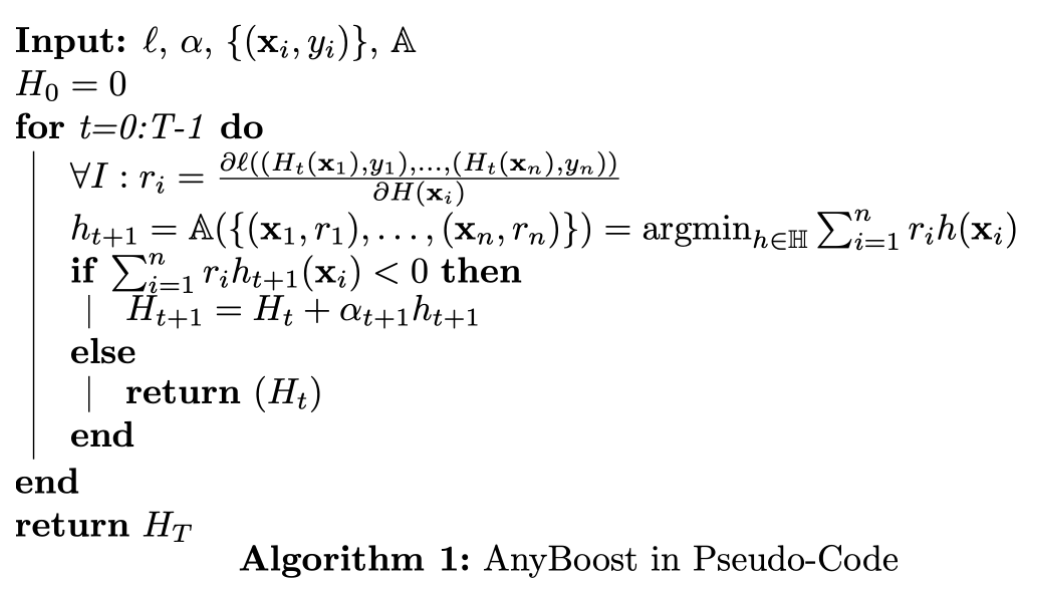
\includegraphics[width=0.5\textwidth]{img/anyboost.png}
\end{figure}

\subsection{AdaBoost}

We begin by describing the most popular boosting algorithm due to
Freund and Schapire (1997) called “AdaBoost”. Consider a two-class
problem where:
\begin{itemize}
    \item The output variable are coded as $y_{i} \in \{ -1, 1\} \; , \forall i $
    \item Weak learners $h \in \mathbb{H}$ are binary, $h(x_{i}) \in \{-1,1\} \; , \forall i$
    \item The loss is the exponential loss: $\ell(H) = \sum_{i=1}^{n} e^{-y_{i}H(x_{i})}$
\end{itemize}

First we compute the gradient $\mathbf{r_{i}} = \dfrac{\partial \ell}{\partial H} (x_{i}) = -y_{i}e^{-y_{i}H(x_{i})} $ \\
For notational convenience, let us define $ \mathbf{w_{i}} = \dfrac{e^{-y_{i}H(x_{i})}}{\sum_{i=1}^{n} e^{-y_{i}H(x_{i})}} $ so that $\sum_{i=1}^{n}w_{i} = 1$.  \\
Each weight $\mathbf{w_{i}}$ therefore has a very nice interpretation: it is the relative contribution of the training point $(x_{i},y_{i})$ towards the overall loss. Now, in order to find the best next weak learner, we need to solve the optimization problem posed earlier:



\begin{equation*}
\begin{aligned}
&   h(x_{i}) = argmin_{h \in \mathbb{H}} \; \sum_{i=1}^{n} r_{i} h(x_{i}) 
  \\
  &= argmin_{h \in \mathbb{H}} \; -\sum_{i=1}^{n} y_{i}e^{-y_{i}H(x_{i})} h(x_{i}) && \text{(substitute in $r_{i}$)}\\
&  = argmin_{h \in \mathbb{H}} \; -\sum_{i=1}^{n} y_{i}w_{i} h(x_{i}) &&  \text{(we can divide by $\sum_{i=1}^{n} e^{-y_{i}H(x_{i})}$ since it is a constant)} \\
& = argmin_{h \in \mathbb{H}} \; \sum_{i: h_(x_{i}) \not = y_{i}} w_{i} - \sum_{i: h_(x_{i})  = y_{i}} w_{i} && \text{( since $h(x_{i})y_{i} = 1 \iff h(x_{i}) = y_{i} $)} \\
& = argmin_{h \in \mathbb{H}} \; \sum_{i: h_(x_{i}) \not = y_{i}} w_{i} && \text{(since $\sum_{i: h_(x_{i}) \not = y_{i}} w_{i} = 1 - \sum_{i: h_(x_{i})  = y_{i}} w_{i}$)}
\end{aligned}
\end{equation*}

Let us denote this weighted classification error as $\epsilon =\sum_{i: h_(x_{i}) \not = y_{i}} w_{i} $. Then, in order for the inner-product $\sum_{i=1}^{n} r_{i}h(x_{i})$ to be negative, it just needs less than $\epsilon<0.5$ weighted training error.\\

The next step is finding the optimal stepsize $\mathbf{\alpha}$ (i.e. the one that minimizes $\ell$ the most). 

We would like to solve the following optimization problem:

$$\alpha = argmin_{\alpha}\; \ell (H+ \alpha h) = argmin_{\alpha}\; \sum_{i=1}^{n} e^{-y_{i}[H(x_{i}) + \alpha h(x_{i})]} $$
We differentiate w.r.t. $\alpha$ and equate with zero: 
\begin{equation*}
\begin{aligned}
&   \dfrac{\partial \ell(H+\alpha h)}{\partial \alpha} = 0 \implies \sum_{i=1}^{n} y_{i}h(x_{i})e^{-(y_{i}H(x_{i}) + \alpha y_{i}h(x_{i}))} = 0
  \\
  & - \sum_{i:h(x_{i})y_{i}=1}  e^{-(y_{i}H(x_{i}) + \alpha \overbrace{y_{i}h(x_{i}}^{1}))} +  \sum_{i:h(x_{i})y_{i} = -1}  e^{-(y_{i}H(x_{i}) + \alpha \overbrace{y_{i}h(x_{i}))}^\text{$-1$}} = 0 && \text{( $y_{i}h(x_{i}) \in \{1,-1\}$)} \\
  & - \sum_{i:h(x_{i})y_{i}=1} w_{i} e^{-\alpha} + \sum_{i:h(x_{i})y_{i} = -1} w_{i} e^{\alpha} = 0 && \text{(divide everything by $\sum_{i=1}^{n} e^{-y_{i}H(x_{i})}$)}\\
  & - (1 - \epsilon) e^{-\alpha} + \epsilon e^{\alpha} = 0 && \text{($\epsilon = \sum_{i: h_(x_{i}) y_{i} = -1} w_{i} $)} \\
  & \alpha = \dfrac{1}{2} \ln {\dfrac{1-\epsilon}{\epsilon}}
\end{aligned}
\end{equation*}

It is unusual that we can find the optimal step-size in such a simple closed form. One consequence is that AdaBoost converges extremely fast. \\

Finally, after you take a step, i.e. $H_{t+1}=H_{t}+ \alpha h$, you need to re-compute all the weights and then re-normalize. It is however straight-forward to show that the unnormalized weight $\hat{w}_{i}$ is updated as:
$$\hat{w}_{i} \leftarrow \hat{w}_{i} e^{-\alpha h(x_{i}) y_{i}} $$ 

and that the normalizer $Z = \sum_{i=1}^{n} e^{-y_{i}H(x_{i})} $ becomes:
\begin{equation*}
\begin{aligned}
&  
  Z^{(t+1)} = \sum_{i=1}^{n} e^{-y_{i}(H(x_{i})+ \alpha h(x_{i}))} = Z^{(t)} \cdot \sum_{i=1}^{n} \dfrac{1}{Z^{(t)}} e^{-y_{i}(H(x_{i})+ \alpha h(x_{i}))} = Z^{(t)} \cdot \sum_{i=1}^{n} w_{i}^{(t)} e^{-y_{i} \alpha h(x_{i})}
  \\
  &  = Z \cdot ( \sum_{i:h(x_{i})y_{i}=1} w_{i}^{(t)} e^{-\alpha} + \sum_{i:h(x_{i})y_{i}=-1} w_{i}^{(t)} e^{\alpha}) = Z^{(t)} \cdot [(1-\epsilon)e^{-\alpha} + \epsilon e^{\alpha} ] \\ 
  & = Z^{(t)} \cdot [(1-\epsilon) \dfrac{\sqrt{\epsilon}}{\sqrt{1-\epsilon}} + \epsilon \dfrac{\sqrt{1-\epsilon}}{\sqrt{\epsilon}}  ] = Z^{(t)} \cdot 2\sqrt{\epsilon (1-\epsilon)}
\end{aligned}
\end{equation*}

$$Z \leftarrow Z \cdot 2 \sqrt{\epsilon (1-\epsilon)}$$

Putting these two together we obtain the following multiplicative update rule:
$$ w_{i} \leftarrow w_{i} \cdot \dfrac{e^{-\alpha h(x_{i}) y_{i}}}{2 \sqrt{\epsilon (1-\epsilon)}}$$

The pseudo-code for AdaBoost will then be the following: 
\\ \\ 
\begin{figure}[h]
\centering
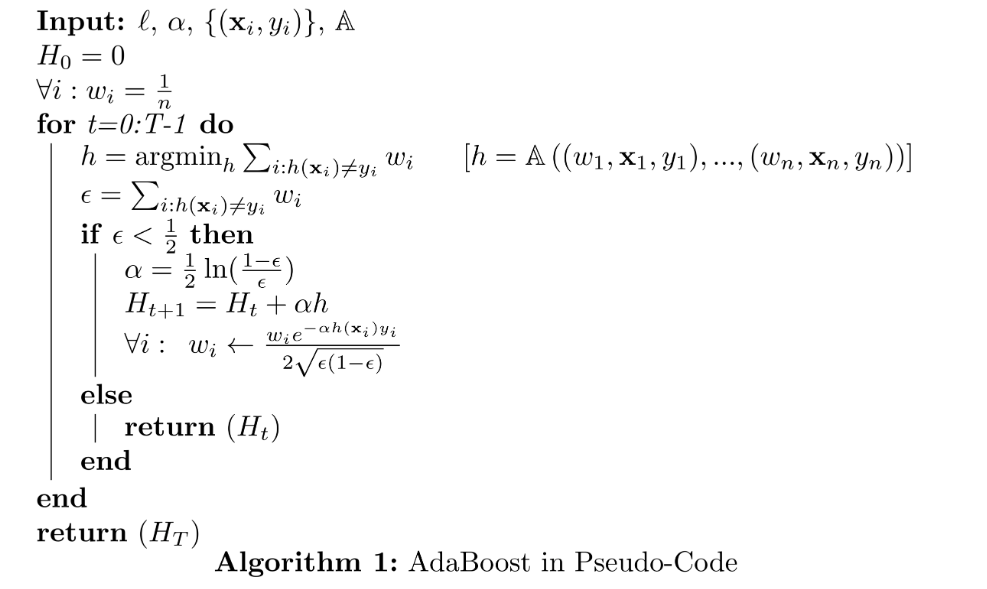
\includegraphics[width=0.9\textwidth]{img/adaboost.png}
\end{figure}

\newpage
Furthermore, we can use the normalizer $Z$ to bound the loss function after $\mathbf{T}$ iterations:

\begin{equation*}
\begin{aligned}
&  
  \ell(H) = Z = Z_{0} \prod_{t=1}^{T}2\sqrt{\epsilon_{t}(1-\epsilon_{t})} = n \prod_{t=1}^{T}2\sqrt{\epsilon_{t}(1-\epsilon_{t})} && \text{($Z_{0}=n$ when all weights are $\dfrac{1}{n}$)}
  \\
  & \leq n \cdot (4 c(1-c))^{\dfrac{T}{2}} && \text{(we define $c = max_{t} \; \epsilon_{t}$)}
  \\ 
  & \leq n \cdot (4 (\dfrac{1}{4} - \gamma^2))^{\dfrac{T}{2}} \leq n \cdot (1 - 4\gamma^2)^{\dfrac{T}{2}} &&  \text{($max_{c} \; c(1-c) = \dfrac{1}{4}  \land c < \dfrac{1}{2} \implies$ this bound: $c(1-c) = \dfrac{1}{4} - \gamma^2$)} \\
   \end{aligned}
\end{equation*}
In other words, $ \ell(H) \leq n \cdot (1 - 4\gamma^2)^{\dfrac{T}{2}}$  tells us that the training loss is \textbf{decreasing exponentially!}
In fact, we can go even further and compute after how many iterations we must have zero training error (note that the training loss is an upper bound on the training error).\\ We can  compute the number of steps required until the loss is less than 1, which would imply that not a single training sample is misclassified:
$$n \cdot (1 - 4\gamma^2)^{\dfrac{T}{2}} < 1 \implies T > \dfrac{2\log{(n)}}{\log{(\dfrac{1}{1-4\gamma^2})}}$$
This is an amazing result! It shows that after $\mathbf{O(\log{n})}$ iterations your training error must be zero. 

\subsection{The Margins Explanation for Boosting’s Effectiveness}

We can visualize the effect AdaBoost has on the margins of the training examples by
plotting their distribution. In particular, we can create a plot showing, for each $\theta \in [-1, +1]$,
the fraction of training examples with margin at most $\theta$. 

\begin{figure}[h]
\centering
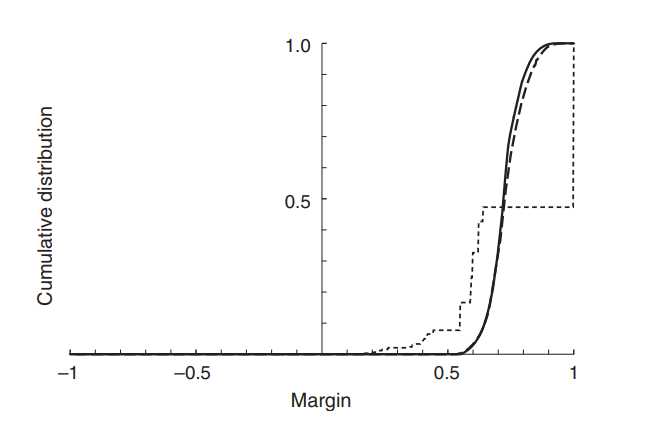
\includegraphics[width=0.5\textwidth]{img/adaboost_margin.png}
\caption{The margin distribution graph for boosting  showing the cumulative distribution of margins of the training instances after 5, 100, and 1000 iterations, indicated by short-dashed, long-dashed (mostly hidden),
and solid curves, respectively. }
\end{figure}

Whereas nothing at all is happening to the training error, these curves expose dramatic changes happening on
the margin distribution. For instance, after five rounds, although the training error is zero
(so that no examples have negative margin), a rather substantial fraction of the training
examples (7.7\%) have margin below 0.5. By round 100, all of these examples have been
swept to the right so that not a single example has margin below 0.5, and nearly all have
margin above 0.6. (On the other hand, many with margin 1.0 have slipped back to the 0.6–0.8
range.) In line with this trend, the minimum margin of any training example has increased
from 0.14 at round 5 to 0.52 at round 100, and 0.55 at round 1000.
\textbf{Thus, this example is indicative of the powerful effect AdaBoost has on the margins,
aggressively pushing up those examples with small or negative margin}. \\ \\
Indeed, as will be seen, AdaBoost can be analyzed theoretically along exactly these lines.
We will first prove a bound on the generalization error of AdaBoost that depends only on the margins of the training examples, and not on the number of rounds of boosting. Thus, this bound predicts that AdaBoost will not overfit regardless
of how long it is run, provided that large margins can be achieved (and provided, of course,
that the base classifiers are not too complex relative to the size of the training set):

\begin{theorem}
Let $\mathcal{D}$ be a distribution over $\mathcal{X} \times \{ -1, +1\}$, and let $\mathcal{S}$ be a sample of $m$ examples chosen independently at random according to $\mathcal{D}$. Assume that the base classifier space
$\mathbb{H}$ is finite, and let $\delta > 0$. Then with probability at least $1 -  \delta$ over the random choice of the
training set $\mathcal{S}$, every weighted average function $f$ satisfies the following bound:
$$\mathbb{P}_{\mathcal{D}}[\overbrace{yf(x)}^\text{margin} \leq 0] \leq  \mathbb{P}_{\mathcal{S}}[yf(x) \leq \theta] + O(\sqrt{\dfrac{\log{\mathbb{|H|}}}{m \theta^2} \cdot log(\dfrac{m \theta^2}{\log{\mathbb{|H|}}} )+ \log{\dfrac{1 / \delta}{m}} }) 
$$
$$\text{for all } \theta > \sqrt{\dfrac{log{\mathbb{|H|}}}{4m}}$$
\end{theorem}

The term on the left is the generalization error. The first term on the right
is the fraction of training examples with margin below some threshold $\theta$. This term will be
small if most training examples have large margin (i.e., larger than $\theta$). The second term on
the right is an additional term that becomes small as the size of the training set $m$ gets larger,
provided the complexity of the base classifiers is controlled for $\theta$ bounded away from zero. \\ \\ The second part of the analysis is to prove that, as observed empirically in Figure 9.1, AdaBoost generally tends to increase the margins of all training examples. 

\begin{theorem}
Given the notation of the previous section, let $\gamma_{t} = \dfrac{1}{2} - \epsilon_{t}$. Then the fraction of training examples with margin at most $\theta$ is at most:
$$\prod_{t=1}^{T} \sqrt{(1+2 \gamma_{t} )^{1+\theta} (1-2 \gamma_{t})^{1-\theta}} $$
\end{theorem}

To get a feeling for this bound, consider what happens when, for all $ \;t,$  $ \epsilon_{t} \leq \dfrac{1}{2} - \gamma $   for
some $\gamma > 0$. Given this assumption, we can simplify the upper bound in theorem 9.3 to:
$$\Big(\sqrt{(1+2 \gamma )^{1+\theta} (1-2 \gamma)^{1-\theta}} \Big)^T$$

When the expression inside the parentheses is strictly smaller than 1, that is, when:
\begin{equation}
    \sqrt{(1+2 \gamma )^{1+\theta} (1-2 \gamma)^{1-\theta}} < 1
\end{equation}

this bound implies that the fraction of training examples with margin  $\leq \theta$ decreases to zero exponentially fast with $T$. Moreover, by solving for $\theta$, we see that equation (9.1)
holds if and only if:

$$\theta < - \dfrac{\log{(1-4 \gamma^2)}}{\log{(\dfrac{1+2 \gamma}{1- 2 \gamma})}}$$

Thus, the margins
of the training examples are guaranteed to be large after a sufficient number of boosting
iterations.\end{document}
